\chapter{Singular Points and Bifurcation}\label{chap5}%5

\section{Introduction}\pageoriginale\label{chap5-sec5.1}%\sec 5.1
 
 First consider the problem in the uniform formulation, viz . 
\begin{equation*}
G(X) =p. \tag{5.2}\label{chap5-eq5.2}
\end{equation*} 
 
 In this formulation we will consider paths which contain singular
 points and give methods to jump over such points. This includes
 bifurcation points in  the general case. 
 
\setcounter{section}{2}
\section{Definition}\label{chap5-eq5.3}

A point $X(s_0)$ on a (smooth) solution path of \eqref{chap5-eq5.2} say, 
$$
\Gamma_{ab} \equiv \left\{ X(s) : X(s) \in  \mathbb{R}^{N+1}, \quad 
G(X)(s))=p, \quad p \in  \mathbb{R}^N, \quad a< s < b \right\}
$$
is a simple singular point if $ s_0 \in  (a,b)$ and Rank
$G_x(X(s_0)) =N-1$.  

Note that here $s$ may be any parameter, it need not be
 arclength. Since $G_X$ is an $N\times (N+1)$ matrix, at a simple
 singular point $X(s_0)$, $G_X$ has two independent null vectors, say,
 $\Phi_1 $ and  $\Phi_2$ in $\mathbb{R}^{(N+1)}$. Without loss of
 generality we can  require  
  $$
 \Phi^T_i \Phi _j= \delta_{ij}; \quad i,j = 1,2,
 $$
 thus introducing an orthogonal system of co-ordinates for $ N\{
 G_X(X(s_0))\}$. Now $G_X^T (X(s_0))$ is an $(N+1) \times N$ matrix of
 rank $N-1$, so that, 
 $$
 N \left\{ G_X^T(X(s_0)) \right\}= \text{span} \{ \psi \},
 $$
 for\pageoriginale some nontrivial $ \psi \in  \mathbb{R}^N$. 
 


\section*{Tangents to $\Gamma_{ab}$}
 
From \eqref{chap5-eq5.2}, it follows that:
$$
G_X(X(s)) \dot{X}(s)=0. 
$$

Hence at $s=s_0$, $\dot{X}(s_0)$ has the form : 
$$
\dot{X}(s_0) = \alpha \phi _1 + \beta \phi_2,  \quad \alpha, \beta
\in  \mathbb{R}. 
$$

Differentiating again we have :
$$
G_X(s)\ddot{X}(s) + G_{XX}(s)\dot{X}(s) \dot{X}(s) = 0. 
$$
 
Now multiplying by $\psi^T$ and evaluating at $s=s_0$, the first
terms vanishes and we have: 
$$
\psi ^T G_{XX}(s_0)\dot{X}(s_0) \dot{X}(s_0)= 0. 
$$
 
Substituting for $\dot{X}(s_0)$, we get :
\begin{equation*}
a_{11} \alpha^2 + 2a _{12}\alpha \beta  + a_{22}
\beta^2=0. \tag{5.4a}\label{chap5-eq5.4a}  
\end{equation*}

Here $a_{ij}$'s are given by:
\begin{equation*}
a_{ij}= \psi^T G_{XX}(s_0) \phi_i \phi_j. \tag{5.4b}\label{chap5-eq5.4b}  
\end{equation*}

Since \eqref{chap5-eq5.4a} is a quadratic equation, it follows that
the roots are governed by  the discriminant: 
\begin{equation*}
\Delta = a^2_{12}-a_{11}a_{22} 
\begin{cases}
> 0,  & \text{ two real roots},\\ 
=0, & \text{ one real root}, \\
<0, & \text{ no real root}. 
\end{cases}\tag{5.4c}\label{chap5-eq5.4c}
\end{equation*}

Since\pageoriginale $\Gamma_{ab}$ is a smooth solution path, it has at
least one nontrivial tangent at each point on $\Gamma_{ab}$. Hence the case
$\Delta < 0$ is not possible. So the following lemma holds. 

\setcounter{chaplemma}{4}
\begin{chaplemma}\label{chap5-lem5.5}
At a simple singular point $X(s_0)$  on a smooth
  solution path $\Gamma _{ab}$ either $ \Delta >0$ or $\Delta = 0$.
\end{chaplemma}

If $\Delta >0$, then  there exist two nontrivial tangents at a
singular point.  This suggests that bifurcation occurs at that
point. Also it gives us an idea for constructing solution paths and
switching over from one branch to another. 

As in the earlier chapter, we adjoin some scalar normalization 
$$ 
N(X,s) =0,
$$
to the equation:
$$
G(X) =0,
$$
where $X \in  \mathbb{R} ^{N+1}$,  $s \in  \mathbb{R}$
to obtain the augmented system from $\mathbb{R}^{N+2} \rightarrow
\mathbb{R}^{N+1}$: 
\begin{equation*}
F(X,s) \equiv
\begin{bmatrix}
G(X)\\
N(X,s)
\end{bmatrix} =0. \tag{5.6a}\label{chap5-eq5.6a}  
\end{equation*}

Using the normalization
\begin{equation*}
N(X,s) = \dot{X}^T (s_0)(X-X(s_0))-(s-s_0), \tag{5.6b}\label{chap5-eq5.6b}   
\end{equation*}
we get: 
\begin{equation*}
F_X(X(s))=
\begin{bmatrix}
G_X (X(s))\\
\dot{X}^T(s_0) 
\end{bmatrix}.\tag{5.6c}\label{chap5-eq5.6c}  
\end{equation*}\pageoriginale
$F_X$ is an $(N+1) \times (N+1)$ matrix. In the previous chapter we
proved that at a simple limit point, the augmented system is
nonsingular (using the normalization in \eqref{chap5-eq5.6b}). 
Although $G_X$ has a two dimensional null space, we will show that
$F_X$ has only one dimensional null space at a simple singular point. 

\setcounter{chaplemma}{6}
\begin{chaplemma}\label{chap5-lem5.7}
$\dim N\{ F_X(X(s_0)\}=1$ at a simple singular point $X(s_0)$ on
    a solution path $ \Gamma_{ab}$. 
\end{chaplemma}

\begin{proof}
We use the notation $F_X(X(s_0)) \equiv F_X(s_0)$ and suppose
$$
F_X(s_0)\phi=0.
$$

Then the first $N$ equations are:
$$
G_X(s_0)\phi=0,
$$
which implies that for some $\alpha_0,\alpha_1  \epsilon\mathbb{R}$: 
$$
\phi =\alpha_0 \Phi_1 +\alpha_1 \Phi_2.
$$

The last equation is :
$$
\dot{X}^{T}(s_0) \phi =0, 
$$
which implies by the orthogonality of $\Phi_1$ and  $\Phi_2$: 
$$
\alpha \alpha_0 + \beta \beta_0 =0.
$$

That\pageoriginale is:
$$
\alpha_0 : \beta_0 = - \beta : \alpha.
$$

This shows that there is, upto a scalar factor, only one null vector
of $F_X(s_0)$. This completes the proof of the lemma.
\end{proof}

We recall that:
$$
\det F_X(s_0)= \prod^{N+1}_{j=1} n_j(s_0), 
$$
where $n_j(s_0)$ are eigenvalues of $F_X(s_0)$. Since $F_X(s_0)$ has a
one dimensional null space at least one of the eigenvalues is zero. We
assume only one is zero. i.e. zero is an algebraically simple
eigenvalues. 
Assume that $n_1(s_0)=0$ and $n_j(s_0) \neq 0$ for $j=2, \ldots
N+1$. Now consider $\det F_X(X)$ for $\parallel X-X(s_0)\parallel$
small and let the corresponding eigenvalues be $n_j(X)$. Suppose 
$$
\nabla_X n_1(X)|_{X=X(s_0)}\neq 0.
$$

Then we can apply the implicit function theorem to show that
$n_1(X)=0$ on a smooth manifold $M$ of dimension $N$. Thus $\det F_X=0$
on $M$. If the solution path is transversal to $M$, i.e. the tangent
at the point of intersection makes an acute angle with the normal to
the manifold, then the path crosses $M$. So the sign of $\det
F_X(X(s))$ changes along the path. Then theorem \ref{chap3-sec3.17}
allows us to conclude that the point of intersection is a bifurcation
point.  

Now we compute the angle between the tangent $X(s_0)$ to $\Gamma_{ab}$
at $s=s_0$ and the normal to the above manifold $M$ at $s=s_0$,
viz.$\nabla_X n_1(X(s_0))$. 
Let\pageoriginale $\phi(X(s))$ denote the eigenvector corresponding to
$n_1(X(s))$. Then  
$$
F_X(s)) \Phi(X(s))=n_1(X(s))\Phi(X(s))
$$

Differentiating this expression and evaluating at $s=s_0$, where $n_1( 
X(s_0))=0$, yields
$$
F_{XX}\dot{X} \Phi+F_X \Phi_X \dot{X} = < \nabla 
n_1, \dot{X} > \Phi 
$$

Let
$$
N \{ F^T_X|_{s=s_0}\} =\text{ span } \{\Psi\}. 
$$

Then taking innerproduct with $\Psi$,
$$
< \Psi, F_{XX}\dot{X} \Phi > = < \nabla n_1, \dot{X} >
<\Psi,\Phi >. 
$$

To evaluate the required angle $< \nabla n_i, \dot{X}>$, we
need to find $\Phi$ and $\Psi$. Lemma \ref{chap5-lem5.7} shows 
$$
\Phi = \beta \Phi_1-\alpha \Phi_2
$$

Also we have
$$
\Psi = (\Psi,0), \qquad \Psi \in N\{G^T_X(X(s_0))\} 
$$
and hence using the notations of (\ref{chap5-eq5.4a},b,c,),
\begin{align*}
< \Psi, F_{XX}\dot{X} \Phi > & = < \Psi, G_{XX}(\alpha \Phi_1 + \beta
\Phi_2)(\beta \Phi_1-\alpha \Phi_2) >\\ 
& =\alpha \beta a_{11}+(\beta^2 - \alpha^2)a_{12}-\alpha \beta
a_{22}\\ 
& = (\beta^2 - \alpha^2)(a_{11}\frac{\alpha}{\beta}+a_{12}) =(\beta^2
- \alpha^2)\surd \Delta 
\end{align*}

Since at $s=s_0$, zero is an algebraically simple eigenvalue of
$F_X(X(s_0))$, 
$$
< \Psi, \Phi > \neq 0.
$$\pageoriginale

Thus we deduce that the required angle is not zero if $\Delta > 0$ and
hence the point $s=s_0$ on the solution path is a bifurcation point. 

By choosing the basis vectors for $N\{G_X(X(s_0))\}$ suitably, the
above computation can be simplified considerably. For example, by
taking 
$$
N\{G_X(X(s_0))\}= \text{ span }\{\Phi_1,\dot{X}\}, 
$$
we get
$$
< \Psi, F_{XX}\dot{X} \Phi > =a_{12}
$$

This is done in detail in the bifurcation theorem below.


\setcounter{section}{7}
\section{Bifurcation Theorem}\label{chap5-sec5.8}%sec 5.8

\textit{Let $X^0 =X(s_0)$ be a simple singular point on a smooth
  solution path} 
$$
\Gamma_{ab}=\{X=X(s) \in \mathbb{R}^{N+1}, \quad G(X(s))=p, p
\in \mathbb{R}^N , \quad s_a <s < s_b \}.
$$

 \textit{Let $\Delta > 0$ and 0 be an algebraically simple
   eigenvalue of $F_X(X(s_0))$ (defined as in \eqref{chap5-eq5.4c} and
   \eqref{chap5-eq5.6c} 
   respectively). Then $X^0$ is a bifurcation point on $ \Gamma_{ab}$} 

\begin{proof}
Consider the system:
\begin{equation*}
F(X,s) \equiv
\begin{bmatrix}
G(X)\\
N(X,s)
\end{bmatrix}
=0
\end{equation*}

Here $s$ is the parameter used to define $\Gamma_{ab}$. We will show
that $F$ has a bifurcation\pageoriginale at $s=s_0$ which in turn will
prove that 
$G$ has a bifurcation at $s=s_0$. Consider the normalization: 
$$
N(X,s) =\dot{X}(s_0)^T [X-X(s_0)]-t(s) 
$$
where $t(s)$ is the distance between $X(s_0)$ and the projection of
$X(s)$ onto the tangent to $\Gamma_{ab}$ at $X(s_0)$. See
Fig.~\ref{chap5-fig5.1}.  

\begin{figure}[H]
\centering
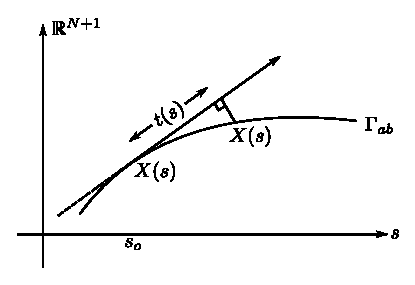
\includegraphics{vol79-fig/fig79-25.eps}
\smallskip
\caption{}
\label{chap5-fig5.1}
\end{figure}

With the indicated normalization, $X(s)$ is a solution of $F(x,s)=0$.
We have :
\begin{equation*}
F_X(X(s))=
\begin{bmatrix}
G_X(s_0)\\
\dot{X}(s_0)^T
\end{bmatrix}
\end{equation*}

At a singular point $G_X$ has a two dimensional null space and the
tangent vector, $\dot{X}(s_0)$, is in $N\{G_X(s_0)\}$. Hence
$\dot{X}(s_0)= \alpha \Phi_1 + \beta \Phi_2$, for some $\alpha$, $\beta
\in \mathbb{R}$. We choose the basis vectors $\Phi_1$ and
$\Phi_2$ of $N\{G_X(s_0)\}$ such that\pageoriginale 
$\alpha = 0$, $\beta=1$. We also
proved that $N\{G_X(s_0)\}$ has dimension one and hence by the choice
of $X(s_0)= \Phi_2$ we must have: 
$$
F_X\{X(s_0)\} \Phi_1=0
$$

Now consider the eigenvalue problem:
$$
F_X(X(s)) \Phi (s)= n(s) \Phi (s).
$$

At $s=s_0$, one of the eigenvalues is zero, say, $n(s_0)=0$ and so
$\Phi(s_0)=\Phi_1$. $F_X$ has a left null vector $\Psi^T$ which is
given by $\Psi^T=(\Psi^T, 0)$ where $\Psi^T$ is a left null vector of
$G^0_X$. Now we can easily show that: 
$$
\dot{n} (s_0)= \frac{\Psi^T F^0_{XX} \Phi_1 \Phi_2}{\Psi^T \Phi_1}=
\frac{a_{12}}{\Psi^T \Phi_1}. 
$$

Since $\alpha = 0$, $\beta=1$ is a root of the equation:
$$
a_{11}\alpha^2 + 2a_{12} \alpha \beta + a_{22} \beta^2 =0 
$$
we must have:
$$
a_{22}=0
$$

Since $\Delta > 0$, this implies that $a_{12} \neq 0$. Hence
$\dot{n}(s_0)\neq 0$. Therefore $\det F_X$ changes sign at $s=s_0$. So
by theorem \ref{chap3-sec3.17}, $F$ and hence $G$ has a bifurcation at
$X(s_0)$.  
\end{proof}

\begin{note*}
This theorem gives conditions under which a point on the solution path
is a bifurcation point. But we do not obtain two smooth branches of
solution. This can be done using the Lyapunov-Schmidt method which we
are not going to discuss here (Refer \cite{key4}, \cite{key26}). 
\end{note*}

Now\pageoriginale consider the parameter formulation of the problem:
\begin{equation*}
G(u,\lambda)=0 \tag{5.9}\label{chap5-eq5.9}
\end{equation*}

\setcounter{section}{9}
\section{Definition}\label{chap5-sec5.10}%sec 5.10

A point $(u(s_0), \lambda(s_0))$ on a solution path $\Gamma_{ab}$ is a
simple singular point if and only if Rank$[G_u(s_0), G_\lambda
  (s_0)]=N-1$. 

At a simple singular point, since Rank $[G_u(s_0), G_\lambda
  (s_0)]=N-1$, $N\{G_u(s_0)\}$ has dimension either one or two. If it
is one then $G_\lambda(s_0)\in R(G_u)$ and if it is two, then
$G_\lambda(s_0) \not \in R(G_u)$. Conversely, if either
$N\{G_u(s_0)\}$ has dimension one and $G_\lambda(s_0)  \in R(G_u)$ or
$N(G_u(s_0))$ has dimension two and $G_\lambda(s_0)  \not \in R(G_u)$,
then $(u(s_0),\lambda(s_0))$ is a simple singular point. So we have 
proven: 

\setcounter{chaplemma}{10}
\begin{chaplemma}\label{chap5-lem5.11}%5.11
The point $(u(s_0), \lambda(s_0))$ is a simple singular point if
  and only if either: 
\begin{equation*}
\begin{array}{r@{\;\;}l}
\text{\rm(i)} &  \dim N\{G_u(s_0)\}=1,\\[4pt]
\text{\rm(ii)}  & G_\lambda (s_0) \in R(G_u). 
\end{array}\tag{5.11a}\label{chap5-eq5.11a}
\end{equation*}
or:
\begin{equation*}
\begin{array}{r@{\;\;}l}
 \text{\rm(i)} & \dim N\{G_u(s_0)\}=2,\\
\text{\rm(ii)}  & G_\lambda (s_0) \in R(G_u). 
\end{array}\tag{5.11b}\label{chap5-eq5.11b}
\end{equation*}
\end{chaplemma}

This case \eqref{chap5-eq5.11b} is similar to the case we discussed in
the uniform 
formulation, since $N(G_u(s_0))$ has two independent null vectors
and\pageoriginale 
we can proceed as above. Now consider the case \eqref{chap5-eq5.11a} and let  
\begin{align*}
N\{G_u(s_0)\} & = \text{ span }\{\Phi\},\\[4pt]
N\{G^T_u(s_0)\} & = \text{ span }\{\Psi\}.
\end{align*}

From (\ref{chap5-eq5.11a}(ii)), the equation:
$$
G_u(s_0)\phi_0=-G_\lambda(s_0),
$$
has a solution and it can be made unique by requiring that $\phi^T
\phi_0=0$. Note that the tangent vector is  
\begin{equation*}
\dot{X}(s_0)=
\begin{bmatrix}
\dot{u}(s_0)\\
\dot{\lambda} (s_0)
\end{bmatrix}.
\end{equation*}

Then we have for some $\alpha$, $\beta \in \mathbb{R}$: 
$$
\dot{\lambda} (s_0)=\beta, \dot{u}(s_0) = \alpha \phi + \beta \phi_0.
$$
where:
\begin{align*}
\dot{X}(s_0) & =\alpha \Phi_1 + \beta \Phi_2 \\
\Phi_1 & = \left(\displaystyle{\mathop{{}^{\phi}_0}} \right), \; 
 \Phi_2 =
\left(\displaystyle{\mathop{{}^{\phi_0}_1}} \right).
\end{align*}

From \eqref{chap5-eq5.9} with $(u,\lambda)=(u(s),\lambda(s))$, we get on
differentiating twice and setting $s=s_0$: 
$$
G^0_u \ddot{u}_0 +G^0_\lambda \ddot{\lambda}_0 + (G^0_{uu} \dot{u}_0
\dot{u}_0 + 2G^0_{u \lambda} \dot{u}_0 \dot{\lambda}_0+G^0_{\lambda
\lambda} \dot{\lambda}_0 \dot{\lambda}_0)=0. 
$$

Multipling by $\Psi^T$, we get,
\begin{equation}
a_{11} \alpha^2 +2a_{12}\alpha \beta +a_{22}\beta^2 =0,
\tag{5.12a}\label{chap5-eq5.12a} 
\end{equation}
where now:
\begin{equation*}
\begin{split}
a_{11} & = \Psi^T G_{uu}(s_0)\phi \phi \\ 
a_{12} & = \Psi^T [G_{uu}(s_0)\phi_0 +G_{u \lambda}(s_0)]\phi\\ 
a_{22} & = \Psi^T [G_{uu}(s_0)\phi_0 \phi_0 +2G_{u
    \lambda}(s_0)\phi_0 +G_{\lambda \lambda}(s_0)]. 
\end{split}\tag{5.12b}\label{chap5-eq5.12b}
\end{equation*}\pageoriginale

Again if $\Delta > 0$, \eqref{chap5-eq5.12a} has two real roots and if
$\Delta = 0$, it has one real root. It can be shown that $\Delta > 0$, then each
root $(\alpha^* , \beta^*)$ of (\ref{chap5-eq5.12a},b) generates a
smooth solution are $(u(s),\lambda(s))$ for $s$ and $s_0$ of the form: 
\begin{align*}
u(s) & =u_0+(s-s_0)[\alpha(s)\phi_0 + \beta(s)\phi_1]+(s-s_0)^2 v(s), \\
\lambda(s) & =\lambda_0+(s-s_0)\alpha(s),
\end{align*}
where,
\begin{align*}
\Psi^T v(s) &=0,\\
\alpha(s_0) &=\alpha^*,\\
\beta(s_0) &=\beta^*.
\end{align*}

For details see \cite{key7}. This result is well known in other forms. See
\cite{key5}, \cite{key26}. 

\setcounter{section}{12}
\section{Continuation Past Simple Singular
  Points}\label{chap5-sec5.13}%sec 5.13 

Let $\Gamma_{ab}=\{X(s):X(s) \in \mathbb{R}^{N+1}, \;  G(X(s))=0,
s_a < s <s_b\}$ be a smooth path. Assume that at $s=s_0 \in
(s_a,s_b)$, the point $X(s_0)$ is an isolated simple singular
point, that is rank of $G_X(X(s))=N$ in the intervals $[s_a,s_0)$
  and $(s_0,s_b]$ and the rank is $N-1$ at $s=s_0$. 

Let\pageoriginale
\begin{equation*}
F(X,s) \equiv
\begin{bmatrix}
G(X)\\
N(X,s)
\end{bmatrix}
=0,
\end{equation*}
where,
$$
N(X,s) \equiv \dot{X}^T(s_a)[X-X(s_a)]-(s-s_a). 
$$

We try to construct a solution using the Newton iteration method : 
\begin{equation*}
\begin{array}{r@{\;\;}>{$}p{7cm}<{$}}
 \text{\rm(a)} & A_U (s) \equiv F_X(X_U (s),s),\\ 
\text{\rm(b)} & A_U (s) [X_{U +1}(s)- X_U (s)] \equiv -F(X_U (s),s),\newline U =
0,1,2, \ldots,  
\end{array}\tag{5.14}\label{chap5-eq5.14}
\end{equation*}
with the initial estimate $X_0(s)$ as:
$$
X_0(s)=X(s_a)+(s-s_a)\dot{X}(s_a).
$$


To assure convergence, we have to show that $X_0(s)$ is in an
appropriate domain of convergence. Recall the Newton-Kantorovich
theorem  \ref{chap2-sec2.23}: we get convergence under the assumptions
that, for some $s\neq s_0$ in $(s_a,s_b)$:
\begin{enumerate}[(a)]
\item $F(X(s),s)=0$,
\item $|| F^{-1}_X(X,(s), s)|| \le \beta(s)$,
\item $|| F_X(X,s)-F_X(Y,s)|| \le \gamma(s) || X-Y ||$, for all $X,Y
  \in B_{\rho(s)}(X(s)),\rho(s)>0$, 
\item $\rho(s) < \dfrac{2}{3 \beta(s)\gamma(s)}$.
\end{enumerate}

Of course as $s \to s_0$, $||F^{-1}_X(X(s),s)|| \to \infty$. But in the
case simple bifurcation point, it can be shown that
$||F^{-1}_X(X(s),s)||\le \dfrac{M_0}{|s-s_0|}$ for some $M_0 >0$, $s
\neq s_0$ (See \cite{key6}). This shows that there is a full conical
neighbourhood,\pageoriginale 
with positive semiangle  about the solution are through
$X(s_0)$, and vertex at $X(s_0)$, in which $F_X (Y,s)$ is
nonsingular. See Figure~\ref{chap5-fig5.2}. 
Note that the tangent $\dot{X}(s_a)$ departs
from one cone at the point $A$ and penetrates at $B$ the other
cone. We have already seen that for all initial values within this
conical neighbourhood, the iterates converge.Hence this allows us to
continue our procedure without any trouble at the singular point. The
point $X(s_0)$ can be determined by a bisection procedure with $s_1 = s_a$
and $s_U < s_0 < s_{U+1}$, for $U= 1,2,3, \ldots$ Each new tangent line
through the new solution $X(s_U)$ will have smaller chord lying
outside the cone. In the limit the tangent through $X(s_0)$ the
bifurcation point, is entirely contained within the cone
(locally). The final configuration or a close approximation to it,
gives one of the best techniques for computing the bifurcation branch
by merely switching the tangent to be used in the normalization. See
Figure~\ref{chap5-fig5.3}. 
We will discuss later in this chapter how to find the new
tangent 
\begin{figure}[H]
\centering
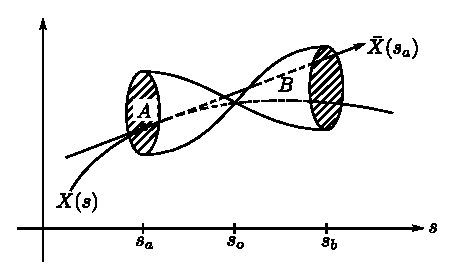
\includegraphics{vol79-fig/fig79-26.eps}
\smallskip
\caption{}
\label{chap5-fig5.2}
\end{figure}
%%%%
\begin{figure}[H]
\centering
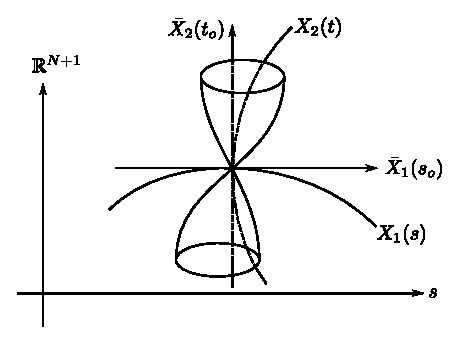
\includegraphics{vol79-fig/fig79-27.eps}
\smallskip
\caption{}
\label{chap5-fig5.3}
\end{figure}\pageoriginale

\setcounter{section}{14}
\section{Properties at Folds and Bifurcation Points on
  Paths}\label{chap5-sec5.15}%\sec 5.15

For the parameter formulation
\begin{equation*}
G(u,\lambda)=p, \tag{5.16}\label{chap5-eq5.16}
\end{equation*}
we consider the eigenvalue problem:
\begin{equation*}
\begin{array}{r@{\;\;}l}
\text{(a)} & G_u(s)\phi(s)=n(s)\phi(s),\\
\text{(b)} & || \phi (s) ||^2 =1.
\end{array}\tag{5.17}\label{chap5-eq5.17}
\end{equation*}
along a solution path of \eqref{chap5-eq5.16}:
$$
\Gamma_{ab} \equiv \{(u(s),\lambda(s)):G(u(s),\lambda(s))=p, \quad s_a
< s < s_b\} 
$$

Note that at an algebraically simple eigenvalue, $\phi(s)$ and $n(s)$
are $C^\infty$ functions\pageoriginale if $G$ is $C^{\infty}$. Assume
that the problem has a simple limit point or a simple singular point of type
\eqref{chap5-eq5.11a} at $s = s_{0} \in (s_{a}, s_{b})$. Then we have:  
\begin{align*}
N \{G^{T}_{u}(s_{0})\} &  = \text{span} \{\psi\}, \\
N \{G_{u}(s_{0})\} &  = \text{span} \{\phi\},
\end{align*}
for some $\psi$, $\phi \in \mathbb{R}^{N}$. Since $G_{u}(s_{0})$ is
singular and the null space is spanned by $\phi$, we must have, for
some $\{\phi (s), n (s)\}$: 
$$
n(s_{0}) = o, \phi (s_{0}) = \phi
$$

Now differentiating (\ref{chap5-eq5.17}a) twice and multiplying by
$\psi^{T}$ and setting $s = s_{0}$, we get: 
\begin{equation*}
\psi^{T}[G_{uu}(s_{0})\dot{u} (s_{0}) \phi + G_{u \lambda}
  (s_{0})\dot{\lambda}
  (s_{0}) \phi] = \dot{n}(s_{0}) \psi^{T}
\phi. \tag{5.18} \label{chap5-eq5.18} 
\end{equation*}

Observe that if the eigenvalue is algebraically simple then $\psi^{T}
\phi \neq 0$. So in this case we can solve for $\dot{n}(s_{0})$. We
use this in the proof of the following lemma.  

\setcounter{chaplemma}{18}
\begin{chaplemma}\label{chap5-lem5.19}
Let $(u(s_{0}), \lambda(s_{0}))$ be a simple quadratic fold on
$\Gamma_{ab}$. Assume that $n (s_{0}) = 0$ is an algebraically simple 
eigenvalue of $G_{u}(s_{0})$. Then $\dot{n}(s_{0}) \neq 0$ and $\det
G_{u}(s_{0})$ changes sign at $s = s_{0}$. 
\end{chaplemma}

\begin{proof}%pro
At a fold point, 
$$
\dot{\lambda}(s_{0}) = 0, \dot{u}(s_{0}) = \phi.
$$

Hence\pageoriginale we have:
$$
\dot{n}(s_{0}) = \frac{\psi^{T}G_{uu}(s_{0}) \phi\phi}{\psi^{T}\phi}
\neq 0, 
$$
because $\ddot{\lambda}(s_{0}) = \frac{\psi^{T}G_{uu}(s_{0})
  \phi\phi}{\psi^{T}G_{\lambda}} \neq 0$ and this implies that
$\psi^{T}G_{uu}(s_{0}) \phi\phi \neq 0$. 
Also if $n_{j}(s)$ are the eigenvalues of $G_{u}(s)$, then, 
$$
\det G_{u}(s) = \prod\limits^{N}_{j=1} n_{j}(s).
$$

Without loss of generality, assume that :
$$
n(s_{0}) = n_{1}(s_{0}), n_{j}(s_{0}) \neq o \forall j = 2, \ldots N.
$$

Since the $n_{j}(s)$ are continuous, $n_{1}(s)$ changes sing at $s =
s_{0}$ and all other $n_{j}(s)$, for $j = 2, \ldots N$ do not change
sign in a neighbourhood of $s_{0}$. Hence the lemma follows    
\end{proof}

\begin{chaplemma}\label{chap5-lem5.20}
Let $(u(s_{0}), \lambda(s_{0}))$ be a simple bifurcation
  points on a smooth path $\Gamma_{ab}$ and $n (s_{0}) = 0$ be an
  algebraically simple eigenvalue of $G_{u}(s_{0})$. Let the
  discriminant $\Delta$ of equation (5.12a) be positive. Then
  $\dot{n}(s_{0}) \neq 0$ and $\det G_{u}(s)$ changes sign at $s =
  s_{0}$ on one or both the branches through the bifurcation point
  $(u(s_{0}), \lambda (s_{0}))$ for which $\dot{\lambda} (s_{0} \neq
  0)$. 
\end{chaplemma}

See figures~\ref{chap5-fig5.4}\,a,b,c. The lemma states that the case shown in
fig.~\ref{chap5-fig5.4}c is not possible, since $\dot{\lambda}(s_{0})$
vanishes on 
both the branches. In fig.~\ref{chap5-fig5.4}a, $\dot{\lambda}(s_{0})
\neq 0 $ on 
both the branches, but in fig.~\ref{chap5-fig5.4}b,
$\dot{\lambda}(s_{0}) \neq 0$ on 
$\Gamma_{+}$ and $\dot{\lambda}(s_{0}) = 0$ on $\Gamma_{-}$ 

\begin{figure}[H]
\centering
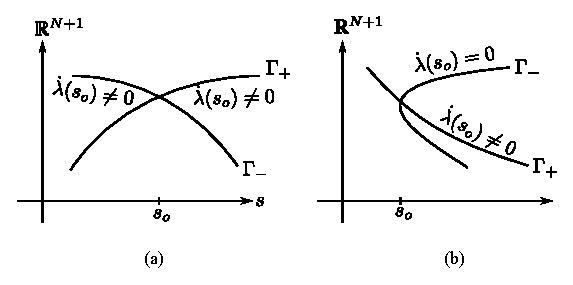
\includegraphics{vol79-fig/fig79-28.eps}

\bigskip
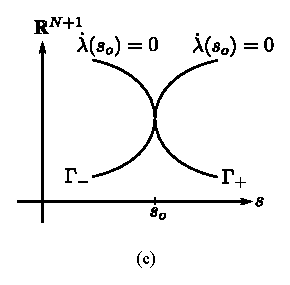
\includegraphics{vol79-fig/fig79-28c.eps}
\caption{}
\label{chap5-fig5.4}
\end{figure}\pageoriginale
%%%


\begin{proof}%pro
Let $(\alpha_{+}, \beta_{+})$ and $(\alpha_{-}, \beta_{-})$ be the
roots of the quadratic equation \eqref{chap5-eq5.12a}. At the bifurcation point,
$\beta_{+}$ and $\beta_{-}$ gives $\dot{\lambda}(s_{0})$ corresponding
to each one of the branches. Therefore if $\dot{\lambda}(s_{0}) = 0$
along one of the branches, then one of $\beta_{+}$, $\beta_{-}$ say
$\beta_{+} = 0$. Then $\alpha_{+}$ cannot be zero. Hence from equation
\eqref{chap5-eq5.12a}, we have     
$$
a_{11} = 0
$$

Since $\Delta > 0$, $a_{12} \neq 0$. Also both $\beta_{+}$ and
$\beta_{-}$ cannot vanish together. Thus at least for one branch
$\dot{\lambda}(s_{0}) \neq 0$. Now for the nonvanishing $\beta$,  
$$
\alpha a_{11} + \beta a_{12} = \beta \sqrt{\Delta} \neq 0. 
$$

From\pageoriginale \eqref{chap5-eq5.18}, we have
$$
\dot{n}(s_{0}) = \frac{\alpha a_{11} + \beta a_{12}}{\psi^{T}\phi}
\neq 0. 
$$

Then $\det G_{u}(s)$ changes sign as in the previous lemma.
\end{proof}

\begin{remark*}%rem
In the case of simple limit points and simple singular points for
which \eqref{chap5-eq5.11a} holds, $N\{G_{u}(s_{0})\}$ has dimension
one. The only 
difference between these two types of points is that in the limit
point case $G_{\lambda} \not \in R(G_{u})$ and in the other
case $G_{\lambda} \in R(G_{u})$. Hence if
$\psi^{T}G_{\lambda}(s_{0}) = 0$, a bifurcation is effected and if
$\psi^{T}G_{\lambda}(s_{0}) \neq 0$, a {\em fold} is effected.  
\end{remark*}

\setcounter{section}{20}
\section{Exchange of Stability}\label{chap5-sec5.21}%sec 5.21

The solutions of \eqref{chap5-eq5.16} are the steady states of the
time dependant 
problems of the form : 
\begin{equation*}
\frac {\partial U}{\partial t} = G(U, \lambda) -
p. \tag{5.22}\label{chap5-eq5.22} 
\end{equation*}

Given an arc of solutions $\{u (s), \lambda(s)\}$ of
\eqref{chap5-eq5.16}, it is 
required to determine the stability of each point as a steady state of
\eqref{chap5-eq5.22}. To use linearized stability theory we seek solutions of
\eqref{chap5-eq5.22} in the form:  
\begin{equation*}
\begin{split}
\lambda & = \lambda (s)\\
U (t,s) & = u(s) + \varepsilon \exp \{tx (s)\} \phi(s)\\
\| \phi (s) \| & = 1.
\end{split}\tag{5.23}\label{chap5-eq5.23}
\end{equation*}

Expanding $G(U(t,s), \lambda(s))$ about $\varepsilon = 0$, we get: 
\begin{equation*}
\frac{\partial U}{\partial t} = G(u(s), \lambda(s)) +
\varepsilon G_{u}(u(s), \lambda(s)) \exp \{tx(s)\} \phi (s) +
0(\varepsilon^{2}). \tag{5.24a}\label{chap5-eq5.24a}
\end{equation*}

But\pageoriginale from \eqref{chap5-eq5.23}, we have :
\begin{equation*}
\frac{\partial U}{\partial t} = \varepsilon n(s) \exp \{tx(s)\} \phi
(s). \tag{5.24b}\label{chap5-eq5.24b}
\end{equation*}

Equating \eqref{chap5-eq5.24a} and \eqref{chap5-eq5.24b}, since
$G(u(s), \lambda(s)) = 0$, it 
follows that: 
$$
n (s) \phi (s) = G_{u}(u(s), \lambda(s)) \phi (s) + 0(\varepsilon).
$$

Hence we are led to the eigenvalue problem :
\begin{equation*}
\begin{array}{r@{\;\;}l}
\text{(a)} & G_{u}(u(s), \lambda (s)) \phi (s) = n (s) \phi (s),\\
\text{(b)} & \| \phi (s) \| = 1. 
\end{array}\tag{5.25}\label{chap5-eq5.25}
\end{equation*}

If all eigenvalues $n = n(s)$ of \eqref{chap5-eq5.25} have Re$(n(s))< 0$ for a
given $s$, we say that $u(s)$ is linearly stable. If at least one
eigenvalue has Re$(n(s)) > 0$, then $u(s)$ is linearly unstable. If
all the eigenvalue have Re$(n(s)) \le 0$, with at least one equality
holding, we say that $u(s)$ is neutrally stable. 

Suppose $(u(s_{0}), \lambda (s_{0}))$ is a limit point as in lemma
\ref{chap5-lem5.19}, then $n(s)$ changes sign as it crosses the point $s =
s_{0}$. Hence if a smooth path of solutions has a simple quadratic
fold at $s = s_{0}$ as in lemma \ref{chap5-lem5.19} 
and solutions for $s > s_{0}$
(or $s < s_{0}$) are stable then they are unstable for $s < s_{0}$ (or
$s > s_{0}$). Hence there is a change of stability at $s =
s_{0}$. Note that here we are not claiming that any branch of
solutions is stable or not. We are only proving that if the solution
branch is stable at one side, then it is unstable on the other
side. We cannot even conclude the converse.   

Similarly\pageoriginale at a bifurcation point as in lemma
\ref{chap5-lem5.20}, $\dot{n}(s_{0}) 
\neq 0$ there and $\det G_{u}(s)$ changes sign at $s = s_{0}$ on one
or both the branches through the bifurcation point for which
$\dot{\lambda} (s_{0}) \neq 0$. Hence here also there may be an
exchange of stability on one or both the branches through the
bifurcation point. Again here observe that we are not proving any
branch of solutions is stable. But we do know that both arcs of one of
the branches cannot be stable.  

\setcounter{section}{25}
\section{Switching Branches at Bifurcation Points}\label{chap5-sec5.26}

Bifurcation points are solutions at which two or more branches of
solutions of  
\begin{equation*}
G(u, \lambda) - p = 0 \tag{5.27}\label{chap5-eq5.27}
\end{equation*}
intersect nontangentially. In this section we consider branch switching
only at simple bifurcation points. For more details see \cite{key19}. 

\medskip
\noindent{\textbf{Method I: }}
An obvious way to determine branches bifurcating at $(u^{0},
\lambda^{0})$ is to determine the two distinct roots of
\eqref{chap5-eq5.12a} and 
use them to determine the distinct tangent vector in : 
\begin{equation*}
\dot{u} = \alpha \phi + \beta \phi_{0}, \dot{\lambda} =
\beta. \tag{5.28}\label{chap5-eq5.28} 
\end{equation*}

Then we can use our pseudoarclength continuation method to determine
the different branches of solutions. If we know one branch of
solutions $\Gamma_{ab}$, then we know the tangent, $(\dot{u}^{0},
\dot{\lambda}^{0})$, to the curve $\Gamma_{ab}$ at $(u^{0},
\lambda^{0})$ and this determines one root of
\eqref{chap5-eq5.12a}. Hence we can 
determine the other tangent easily. Also note that in finding the
values of the coefficients $a_{ij}$ of \eqref{chap5-eq5.12a} we need the
derivatives $G^{0}_{uu}$, $G^{0}_{u \lambda}$ and $G^{0}_{\lambda
  \lambda}$. But we can use the\pageoriginale 
following approximation to these
quantities which avoids the need for determining the second derivatives
of $G$.  
\begin{align*}
a^{\varepsilon}_{11} & = \frac{1}{\varepsilon} \psi^{T} [G_{u}(u^{0} +
  \varepsilon \phi , \lambda^{0}) - G_{u}(u^{0}, \lambda^{0})] \phi,
\\ 
& = a_{11} + 0(\varepsilon), \\ 
a^{\varepsilon}_{12} & = \frac{1}{\varepsilon} \psi^{T} \{[G_{u}(u^{0}
  + \varepsilon \phi_{0} , \lambda^{0}) - G_{u}(u^{0}, \lambda^{0})]
\phi, \\
& \qquad + [G_{\lambda}(u^{0} + \varepsilon \phi , \lambda^{0}) -
  G_{\lambda}~(u^{0},\lambda^{0})]\}, \\ 
& = a_{12} + 0(\varepsilon)\\ 
a^{\varepsilon}_{22} & = \frac{1}{\varepsilon} \psi^{T} \{ G_{u}(u^{0}
+ \varepsilon \phi_{0} , \lambda^{0}) - G_{u}(u^{0}, \lambda^{0})]
\phi_{0} \\
& \qquad + 2[G_{\lambda} (u^{0} + \varepsilon \phi_{0}, \lambda^{0}) -
  G_{\lambda} (u^{0}, \lambda^{0})]\\ 
& \qquad + [G_{\lambda} (u^{0}, \lambda^{0}
  + \varepsilon ) - G_{\lambda} (u^{0}, \lambda^{0})]\},\\ 
&= a_{22} + 0 (\varepsilon).
 \end{align*} 

 Here $\phi, \psi$ and $\phi_{0}$ are nontrivial solutions of  
 $$
 G^{0}_{u} \phi = 0; \quad G^{o^{T}}_{u}\psi = 0; \quad G^{0}_{u}\phi_{0} = -
 G^{0}_{\lambda}, \quad \phi^{T} \phi_{0} = 0. 
 $$

\medskip
\noindent{\textbf{Method II:}}
In this method we assume that one branch through the bifurcation point
has been determined. Then the tangent $(\dot{u}(s_{0}), \dot{\lambda}
(s_{0}))$ can also be assumed to be known on this branch. The idea is
to seek solutions on some subset parallel to the tangent but displaced
from the bifurcation point in a direction normal to the tangent but
in a specific plane. This method avoids the need to evaluate the
coefficients $a_{ij}$, $i,j = 1,2$. Refore \cite{key19}.

The\pageoriginale solution branch $(u_{1}(s), \lambda_{1}(s))$ has a
tangent in the 
direction given by \eqref{chap5-eq5.28}. An orthogonal to this tangent in the
plane spanned by $(\phi, 0)$ and $(\phi_{0}, 1)$ is given by
\eqref{chap5-eq5.28} but with $\alpha$, $\beta$ replaced by: 
$$
\hat{\alpha} = \beta (1 + \| \phi_{0} \|^{2}), \hat{\beta} = -
\alpha\| \phi\|^{2}.  
$$

Then we seek solutions in the form :
\begin{equation*}
\begin{split}
u_{2} & = u_{1}(s_{0}) + \varepsilon(\hat{\beta}\phi_{0} +
\hat{\alpha}\phi_{1}) + v, \\
\lambda_{2} & = \lambda_{1}(s_{0}) + \varepsilon \hat{\beta} + \eta. 
\end{split}\tag{5.29a}\label{chap5-eq5.29a}
\end{equation*}

These are to satisfy:
\begin{equation*}
\begin{split}
G(u_{2}, \lambda_{2}) & = p,\\
N(u_{2}, \lambda_{2}) & \equiv (\hat{\beta}\phi^{T}_{0} + \hat{\alpha}
\phi^{T})_{v} + \hat{\beta}\eta = 0.  
\end{split}\tag{5.29b}\label{chap5-eq5.29b}
\end{equation*}

We use Newton's method to solve \eqref{chap5-eq5.29b} for $v \in
\mathbb{R}^{N}$ and $\eta \in \mathbb{R}$ with the initial estimate
$(v_{0}, \eta_{0}) = (0,0)$. Here $\varepsilon$ much be taken
sufficiently large so that the scheme does not return to
$(u_{1}(s_{0}), \lambda_{1}(s_{0}))$ as the solution.  


\medskip
\noindent{\textbf{Method III (Lyapunov-Schmidt): }}
Another way to determine a branch bifurcating from a known branch
$(u(s), \lambda (s))$ at $s = s_{0}$ is to apply a constructive
existence theory, as in \cite{key22}. We seek the bifurcated branch in the
form :   
\begin{equation*}
\begin{split}
u & = u_{1} (\sigma) + \varepsilon(\phi + v),\quad \psi^{T}v =
0\\
\lambda & = \lambda_{1}(\sigma). 
\end{split}\tag{5.30a} \label{chap5-eq5.30a}
\end{equation*}

Then we have:
\begin{equation*}
 G^{0}_{u}v - \frac{1}{\varepsilon} G(u_{1}(\sigma) + \varepsilon
 (\phi + v), \lambda_{1}(\sigma)), \psi^{T}v =
 0.\tag{5.30b}\label{chap5-eq5.30b}  
\end{equation*}\pageoriginale

To ensure that the right hand side is in $R(G^{0}_{u})$, we try pick
$\sigma = s$ such that $h(s, \varepsilon, v) = 0$, where,   
\begin{equation*}
h(s, \varepsilon, v) = 
\begin{cases} 
\psi^{T}[G^{0}_{u}v - \frac{1}{\varepsilon} G(u_{1}(s) + \varepsilon
  (\phi + v), \lambda_{1}(s))], \varepsilon \neq 0,\\ 
\psi^{T}[G^{0}_{u}v - G(u_{1}(s), \lambda_{1}(s))  (\phi + v)] ;
\varepsilon = 0. 
\end{cases}\tag{5.30c}\label{chap5-eq5.30c}
\end{equation*}

It follows that $h(s_{0}, 0, 0) = 0$ and 
$$
h^{0}_{s} = h_{s}(s_{0}, 0, 0) =
-\psi^{T}[G^{0}_{uu}\dot{u}_{1}(s_{0}) + G^{0}_{u} \lambda
  \dot{\lambda}_{1} (s_{0})] \phi 
$$

Then if $h^{0}_{s} \neq 0$ the implicit function theorem gives the
function\break $s = \sigma (\varepsilon, v)$ and then it can be shown that
\eqref{chap5-eq5.30b} has a unique solution $v = v(\in)$ for
$|\varepsilon|$ sufficiently small, using the contraction mapping
theorem. 

The main difficulty in applying this method is in solving $h(s,
\varepsilon, v) = 0$ for $s$ at each $v = v_U$. If course if
$\lambda$ occurs linearly in the problem and it is used as the
parameter $s$, then this is easy. But in the case, modifications must
be introduced. See \cite{key3}, \cite{key8}. 
This method has also been used for bifurcation from the trivial
branch. See \cite{key31}.   

\medskip
\noindent{\textbf{Method IV: }}
Here we use a technique based on a modification of the Crandall and
Rabinowitz \cite{key5} proof of bifurcation. Thus we seek solutions of the
form \eqref{chap5-eq5.30a} and define  
\begin{equation*}
\begin{split}
\text{(a)} & g (v,s,\varepsilon)  =
\begin{cases}
\frac{1}{\varepsilon} G (u_1(s) + \varepsilon (\phi +v), \lambda_1
(s)) \quad \text{if} \quad \varepsilon \neq 0\\ 
G_u (u_1(s), \lambda_1 (s)) (\phi + v) \quad \text{if} \quad
\varepsilon  =0\\  
\end{cases}\\
\text{(b)} & N(v,s, \varepsilon)  = \psi^Tv.  
\end{split}\tag{5.31}\label{chap5-eq5.31}
\end{equation*}\pageoriginale

Note that 
$$
g(0,s_0,0) = 0, \quad N(0,s_0,0) =0
$$
and 
$$
A^0 = \left. \frac{\partial(g,N)}{\partial(v,s)}
\right|_{0,s_0,0)}=
 \begin{bmatrix}
   G^0_u & B^0 \\
 \psi^T &  0 
\end{bmatrix}, 
$$
where,
$$
B^0 \equiv \left[G^0_{u u } \dot{u_1} (s_0) + G^0_{u \lambda}
  \dot{\lambda_1} (s_0) \right] \phi. 
$$

If $\psi^T B^0 \neq 0$, the by the lemma \ref{chap4-lem4.9}, $A^0$ is
nonsingular. Now 
the implicit function theorem shows that :  
\begin{equation*}
\begin{split}
g(v,s,\varepsilon) & = 0,\\
N(v,s,\varepsilon) & = 0. 
\end{split}\tag{5.32}\label{chap5-eq5.32}
\end{equation*}
has a smooth solution $(v(\varepsilon), \rho (\varepsilon))$ for each
$|\varepsilon| \leq \varepsilon_0$ and using this solution in
(\ref{chap5-eq5.31}a) yields the bifurcating branch of solutions. In solving
\eqref{chap5-eq5.32} we never use $\varepsilon = 0$ so that even when applying
Newton's method, second derivatives need not be computed. 

\medskip
\noindent{\textbf{Method V (Perturbed Bifurcation) :}}
Observe that at a bifurcation point $(u^0, \lambda^0),p$ is not a
regular value for $G$. Since the set of all regular values is dense,
the idea of this method is to perturb $p$, say $p+ \tau q$, $q
\in \mathbb{R}^N$, $||q||= 1$, $\tau \neq 0$, so that $p +
\tau q $ is a regular value for $G$.   
Consider\pageoriginale 
the two smooth branches of solutions through the bifurcation
point $(u^0,\lambda^0)$. If we delete a small neighbourhood of
$(u^0,\lambda^0)$, we obtain 4 different branches of solutions, say
$\Gamma_1$, $\Gamma_2$, $\Gamma_3$, $\Gamma_4$. Then consider the
perturbed problem :   
\begin{equation*}
G(u,\lambda) = p+ \tau q , \quad q \in \mathbb{R}^N, \quad || q|| = 1,
\quad \tau \neq 0. \tag{5.33}\label{chap5-eq5.33} 
\end{equation*}

Assuming $p + \tau q$ is a regular value, this has no bifurcation and
$\Gamma_i$, $i = 1,2,3,4$ will simply be perturbed and will yield smooth
nearby branches of solutions of \eqref{chap5-eq5.33}. These branches can be
connected in 3 ways. See Figs.~\ref{chap5-fig5.5}\,a,b,c. 

\medskip
\noindent
{\bf Case (i)~:}
 Here if we are starting from a solution on $\Gamma_1$, we will get a
 perturbed solution on $\Gamma'_1$ and then we can continue along
 $\Gamma'_1$ to $\Gamma'_4$ which is the perturbed branch of
 $\Gamma_4$. Similarly from $\Gamma_2$, we will obtain $\Gamma'_2$ and
 $\Gamma'_3$ [Fig.~\ref{chap5-fig5.5}a]. 
\smallskip

\noindent
{\bf Case (ii)~:}
In a similar manner we can handle this case also (see
Fig.~\ref{chap5-fig5.5}b).  

\noindent
{\bf Case (iii)~:}
In the cases (i) and (ii) we can determine the other branches
  without any difficulty. Our claim is that the case (iii) doesn't
  happen. To see this we have to study further about fold following
  which we are going to describe in the next section. There we will
  consider the problem \eqref{chap5-eq5.33} as a two parameter, 
$(\lambda,\tau)$ problem and will give an algorithm to obtain a fold . 

\begin{figure}[H]
\centering
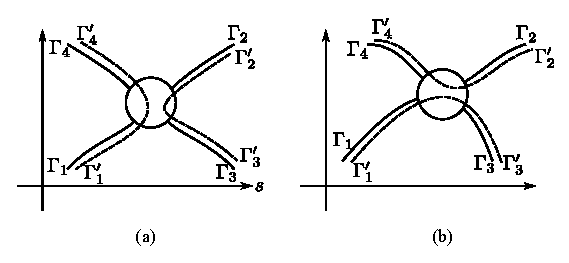
\includegraphics{vol79-fig/fig79-29ab.eps}

\bigskip
\smallskip

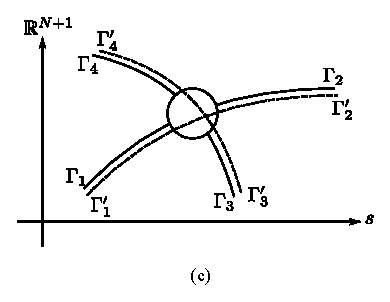
\includegraphics{vol79-fig/fig79-29c.eps}

\smallskip
\caption{}\label{chap5-fig5.5}
\end{figure}\pageoriginale

\section{Multi Parameter Problems (Fold
  Following)}\label{chap5-sec5.34}\pageoriginale%sec 5.34  

We recall the two examples described in the introductory chapter on
population dynamics. We examined the steady state solutions of: 
\begin{align*}
\frac{d \xi}{dt} & = - \xi^2 + \lambda \xi + \tau,\\
\frac{d \xi}{dt} & = - \xi^3 + \lambda \xi + \tau , 
\end{align*}
that is the solution of:
\begin{align*}
{\rm(1)} \quad & - \xi^2+ \lambda \xi + \tau=0,\\
{\rm(2)} \quad & - \xi^3+ \lambda \xi + \tau=0,
\end{align*}

\setcounter{exam}{0}
\begin{exam}\label{chap5-exam1}%%% exam 1
$-\xi^2+\lambda \xi + \tau =0$.

We note that in the $(\lambda, \tau )$ plane there is a curve across
which the number of solutions change. This curve is a fold. See the
solution surface sketched in fig.~\ref{chap1-sec1.2-fig1.4}. 
\end{exam}

\begin{exam}\label{chap5-exam2}%%% exam 2
$-\xi^3+ \lambda \xi + \tau=0$,

In Fig.~\ref{chap1-sec1.2-fig1.8} we show a curve in the $(\lambda,
\tau)$ plane which has 
a cusp at the origin; as $(\lambda, \tau)$ crosses this curve the
number of solutions changes. Look at the solution surface in 
Fig.~\ref{chap1-sec1.2-fig1.12}. This curve is a fold on the solution surface. 
\end{exam}

Hence determining a fold is very important. Other interesting
phenomena may occur along the folds. The solutions lie either to the
left of the fold curve or to the right of the fold curve. In the
latter case, (Fig.~\ref{chap5-fig5.6}a) the fold point is known as a hyperbolic
point and in the former case\pageoriginale (Fig.~\ref{chap5-fig5.6}b)
it is called an elliptic 
point. Suppose the fold point is at $(u_0, \lambda_0, \tau_0)$. In the
elliptic case if $\tau> \tau_0$ we have no solution and on the other
hand if $\tau < \tau_0$, we obtain a closed loop of solutions. A
closed loop of solutions is known as an `isola'. In the second case as
$\tau$ changes from $\tau_0$ we get different branches of
solutions. For a unified theory of perturbed bifurcation and isola
formation see \cite{key21}. 

\begin{figure}[H]
\centering
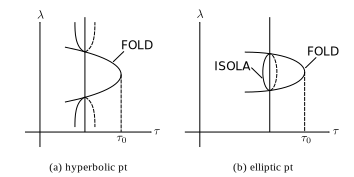
\includegraphics{vol79-fig/fig79-30.eps}
\smallskip
\caption{}\label{chap5-fig5.6}
\end{figure}

Now let $\tau = \tau_0$ and assume that there is a simple quadratic
fold with respect to $\lambda$ at $(u_0, \lambda_0)$. We have $G(u_0,
\lambda_0, \tau_0)=p$ and 
\begin{equation*}
\begin{array}{r@{\;\;}l}
\text{(a)} & N(G_u^{0})= \text{span\,} 
 \{\phi_0\}, \text{ \ for some\ } \phi_0
\neq 0,\\ 
\text{(b)} & G_{\lambda}^{0} \notin R(G_u^{0})=\{v \in
\mathbb{R}^N :\psi_0^Tv=0 \}. 
\end{array}\tag{5.35}\label{chap5-eq5.35} 
\end{equation*}

Here $\psi_0$ is a nontrivial solution of: 
\begin{equation*}
\text{(c)}~G_u^{0 T}\psi _0=0, \tag{5.35}\label{chap5-eq5.35c}
\end{equation*}\pageoriginale
and at a simple quadratic fold:
\begin{equation*}
\text{(d)}~ a=\psi_0^T G^{0}_{uu} \phi _0 \phi_0 \neq
0. \tag{5.35}\label{chap5-eq5.35d} 
\end{equation*}

Now consider the extended system:
\begin{equation*}
F_1(u, \psi. \lambda, \tau) \equiv 
\begin{bmatrix}
G(u, \lambda , \tau)-p \\ 
\psi ^T G_u(u, \lambda, \tau)\\ 
\psi ^T G_\lambda^{0}-1 
\end{bmatrix}=0.
\end{equation*}

Here $F_1: \mathbb{R}^{2N+2} \to \mathbb{R}^{2N+1}$. This system can
be written as: 
\begin{equation*}
\text{(a)}~ F(U, \tau )=0,\tag{5.36}\label{chap5-eq5.36a}
\end{equation*}
where
\begin{equation*}
\text{(b)}~ U= \begin{bmatrix}
u\\ \psi \\ \lambda
\end{bmatrix}
\tag{5.36}\label{chap5-eq5.36b}
\end{equation*}
and $F \equiv F_1$. Note that $(u_0, \psi_0, \lambda_0, \tau_0)$ is a
solution of this system. We use another formulation: 
\begin{equation*}
F_2(u, \psi , \lambda, \tau) \equiv
\begin{bmatrix}
F(u, \lambda, \tau)-p \\
 G_u(u, \lambda. \tau)\phi \\ 
\ell^T\phi-1
\end{bmatrix}=0,\tag{5.37a}\label{chap5-eq5.37a}
\end{equation*}
where $\ell$ is such that
\begin{equation*}
\ell^T \phi_0=1. \tag{5.37b}\label{chap5-eq5.37b}
\end{equation*}

This\pageoriginale can also be written in the form \eqref{chap5-eq5.36a} with $F
\equiv F_2$. In this letter case, we have the following theorem 

\setcounter{chapthm}{37}
\begin{chapthm}\label{chap5-thm5.38} %%% 5.38
At a simple quadratic fold $(u_0. \lambda_0, \tau _0)$:
$$ 
\left. F_{\dot{U}}^{0}= \frac{\partial F}{\partial (u, \Phi , \lambda)}
\right|_{(u_0, \Phi_0,\lambda_0)}= 
\begin{bmatrix}
 G_u^{0} & 0 &G_{\lambda}^{0}\\
 G^{0}_{uu}\Phi _0 & G_u^{0} & G^{0}_{u \lambda} \Phi _0\\
0 & \ell^T & 0\\
\end{bmatrix}
$$
is nonsingular.
\end{chapthm}

\begin{proof}%pro
Assume $F^0_U \Phi =0$, for some $\Phi= \begin{bmatrix} p
  \\q\\r\end{bmatrix}  \in \mathbb{R}^{2N+1}$ 

That is 
\begin{equation*}
\begin{array}{r@{\;\;}l}
\text{(a)} & G^0_Up+ r G^0_{\lambda} =0,\\ 
\text{(b)} & G^0_{uu} \Phi_0 p + G^0_uq + G^0_{u \lambda}\Phi_0
r=0,\\ 
\text{(c)} & \ell^T_q =0.
\end{array}\tag{5.39}\label{chap5-eq5.39}
\end{equation*}

Multiplying (\ref{chap5-eq5.39}a) by  $\psi^T_0$ and using
(\ref{chap5-eq5.35}\,b,c), we get 
$r=0$. Hence $G^0_u p=0$. This  shows that $p= \alpha \Phi _0$, for
some $\alpha \in \mathbb{R}$. So (\ref{chap5-eq5.39}b) implies that  
$$
\alpha \psi^T_0 G^0_{uu} \Phi _0 \Phi_0 = \alpha a=0. 
$$

So that by (\ref{chap5-eq5.35}d), $\alpha$ and hence $p=0$. This implies
$G^0_uq=0$. Hence $q= \beta\Phi _0$ for some $\beta \in
\mathbb{R}$. But by (\ref{chap5-eq5.39}c) we get $\beta \ell^T \Phi_0 =0$. Hence
by \eqref{chap5-eq5.37b}, $\beta$ and $q=0$ 
\end{proof}

Now we can apply the implicit function theorem to obtain 
\begin{align*}
u &= u(\tau)\\
\Phi &= \Phi(\tau)\\
\lambda &=\lambda (\tau)
\end{align*}\pageoriginale
for $| \tau- \delta| < \delta$, for  some $\delta >0$. The arc $( u
(\tau), \lambda (\tau), \tau) \in \mathbb{R}^{N+2,}$, $\tau
\in(\tau_0 - \delta, \tau_0 + \delta)$ is part of the fold
curve. We can also use some other  parametrization, $s$, to to obtain
the solution in the form: 
\begin{align*}
u &= u(s)\\
\Phi &= \Phi(s)\\
\lambda &= \lambda(s)\\
\tau &=\tau(s).
\end{align*}

Now we will show how to use the Bordering Algorithm to find the Newton
iterates applied to solve \eqref{chap5-eq5.37a}. The linear system has
the form:  
\begin{equation*}
LX = 
\begin{bmatrix}
 \underset{\sim}{g} \\
 \gamma 
\end{bmatrix}
\tag{5.40} \label{chap5-eq5.40}
\end{equation*}

Here
$$
L \equiv F_U \equiv 
\begin{bmatrix} 
\tilde{A} & \underset{\sim}{b}  \\
 \underset{\sim}{c}^T & 0 
\end{bmatrix},  \quad 
X \in
\mathbb{R}^{2N+2},\underset{\sim}{g} \in \mathbb{R}^{2N},
\gamma \in \mathbb{R},  
$$
where   
$$
\tilde{A} \equiv 
\begin{bmatrix}
 A & 0\\ 
B & A 
\end{bmatrix} \text{  with } A=  G^0_u, \; B= G^0_{uu} \Phi_0. 
$$

First solve:
\begin{align*} 
& \tilde{A} \underset{\sim}{v}= \underset{\sim}{b},\underset{\sim}{b},
\underset{\sim}{v} \in \mathbb{R}^{2N},\\ 
& \tilde{A} \underset{\sim}{\omega}=
\underset{\sim}{g},\underset{\sim}{g}, \underset{\sim}{\omega}
\in \mathbb{R}^{2N}. 
\end{align*}\pageoriginale

Then form:
$$
\xi = \frac{\gamma-\underset{\sim}{c}^T 
  \underset{\sim}{\omega}}{\underset{\sim}{c}^T \underset{\sim}{v}},  
$$
and 
$$
\underset{\sim}{x} =\underset{\sim}{\omega}- \xi \underset{\sim}{v}.
$$
 
 Note that the system:
 $$
  \tilde{A} \begin{bmatrix}y_1 \\ y_2 \end{bmatrix}
  \equiv \begin{bmatrix}A & 0 \\ B & A \end{bmatrix} \begin{bmatrix}
    y_1 \\y_2 \end{bmatrix} = \begin{bmatrix} \gamma_1
    \\ \gamma_2 \end{bmatrix}, 
 $$
 can easily be solved as follows:
 
 First solve
 $$
  Ay_1 = \gamma_1,
 $$
 and then 
 $$
 Ay_2 = \gamma_2 -By_1.
 $$
 
 Hence it follows that the system \eqref{chap5-eq5.40} can be solved
 by solving  four systems the same coefficient matrix $A$. So we need
 do only one 
 $LU$ decomposition of $A$ and then four backsolves. See the
 Ref. \cite{key33} and also \cite{key15}. 
 
\setcounter{section}{40}
\section{Paths of Periodic Solutions and Hopf
  Bifurcation}\label{chap5-sec5.41}\pageoriginale%sec 5.41 
 
 In this section we will discuss the periodic solutions of the system
 of ODE depending on a parameter: 
  \begin{equation*}
\frac{dy}{dt}= f(y, \lambda). \tag{5.42}\label{chap5-eq5.42}
  \end{equation*} 
  
  First we will briefly describe Poincare's method for containing
  periodic solution branches and then we discuss Hopf bifurcation. We
  do not give a detailed description of these things. A good reference
  for Hopf bifurcation is \cite{key25}. 
  
  We seek periodic solutions of \eqref{chap5-eq5.42}. Suppose for $\lambda =
  \lambda^0$ that $\underset{\sim o}{y}(t)$ satisfies \eqref{chap5-eq5.42} and
  $\underset{\sim o}{y}(t+T^0) = \underset{\sim o}{y}(t)$, for some
  $T^0 > 0$ and  for all $t$. Then $\underset{\sim o}{y} (t)$ is a
  periodic solution (5.42). Since this system is autonomous, for any
  $\sigma$, the translation of $\underset{\sim o}{y} (t)$. viz. 
  $$
  \underset{\sim}{y} (t) = \underset{\sim o}{y}(t+\sigma), 
  $$
  is also a periodic solution. We seek  periodic solution when
  $\lambda$ is pertubed from $\lambda^0$ 
  
  Substituting  $\underset{\sim o}{y} (t)$ in \eqref{chap5-eq5.42} and
  differentiating we get: 
  $$
  \frac{d}{dt} \underset{\sim o}{\dot{y}} (t) = [f_y (\underset{\sim
      o}{y} (t), \lambda^0)] \underset{\sim o}{\dot{y}} (t). 
  $$
  
  Let
  $$
  A_0 (t) = [f_y(\underset{\sim o}{y} (t), \lambda^0)].
  $$
  
  Then we can write 
  $$
  [\frac{d}{dt}- A_0(t)] \underset{\sim 0}{\dot{y}}(t) =0.
  $$\pageoriginale

  Hence the linearised operator $\dfrac{d}{dt}-A_0 (t)$ has a
  nontrivial periodic solutions $\underset{\sim 0}{\dot{y}}(t)$. In
  the case of nonautonomous system this is not in general true. Then
  we have to assume that $f(t,y,\lambda)$ is periodic, with period
  $T(\lambda)$. Then in general the linearized problem does not have
  nontrivial periodic solution and the continuation in $\lambda$ can
  be done yielding solutions with period $T(\lambda)$. In our case
 \eqref{chap5-eq5.42}, $f$ has all possible periods in $t$. 
  
  Consider the periodic solution $\underset{\sim 0}{y}(t)$ of
  \eqref{chap5-eq5.42}. At $t=t_0 =0, \underset{\sim 0}{y}(0)$ is some
  arbitrary point in $\mathbb{R}^N$ and let $\pi \subset \mathbb{R}^N$ be the
  plane which is perpendicular to the tangent, $\underset{\sim
    0}{\dot{y}}(0)$ at $y_0(0)$. That is:   
  $$
  \pi = \{ \underset{\sim}{\xi} \in \mathbb{R}^N:
  \underset{\sim o}{\dot{y}}(0)^T ( \underset{\sim}{\xi}-
  \underset{\sim o}{y}(0)) =0 \} 
  $$
  
  Consider any point $\underset{\sim}{\xi} \varepsilon \pi$ in some
  small neighbourhood of $\underset{\sim o}{y}(0)$ and look at the
  solution curve of \eqref{chap5-eq5.42} passing through this point
  $\underset{\sim}{\xi}$. Suppose the curve intersects this plane
  $\pi$ after sometime, then this point  of intersection is the image
  of $\underset{\sim}{\xi}$ under the poincare map. For the existence
  of Poincare map see \cite{key25}. From the definition  it is clear that
  the periodic solution of \eqref{chap5-eq5.42} corresponds to the fixed points
  of the Poincare map.   
  
  Consider the initial value problem:
  \begin{equation*}
\begin{array}{r@{\;\;}l}
\text{(a)}  & \frac{dy}{dt} =  \frac{f(y, \lambda)},\\
 \text{(b)} & \underset{\sim}{y}(0)= \underset{\sim}{\xi} \in
 \mathbb{R}^N. 
\end{array}\tag{5.43}\label{chap5-eq5.43} 
  \end{equation*}
  
  Let\pageoriginale $\underset{\sim}{y}= \underset{\sim}{y}(t,
  \underset{\sim}{\xi} 
  , \lambda)$ be the solution of \eqref{chap5-eq5.43}, for
  $(\underset{\sim}{\xi}, 
  \lambda) \in B_\rho (\underset{\sim o}{y}(0), \lambda^0)$
  for some $\rho > 0$. The problem thus reduced to: find
  $\underset{\sim}{\xi}$ and $T$ such that : 
  \begin{equation*}
\begin{array}{r@{\;\;}l}
\text{(a)} & \underset{\sim}{y}(T,  \underset{\sim}{\xi}, \lambda) -
\underset{\sim}{\xi} =0,\\ 
\text{(b)} & \underset{\sim o}{\dot{y}} (0)^T [\underset{\sim}{\xi}-
  \underset{\sim o}{y}(0)]=0.  
\end{array}\tag{5.44}\label{chap5-eq5.44}
  \end{equation*}

  These are $(N+1)$ equations in $N+1$ unknowns. Observe that
  at $\lambda = \lambda^0$, we have the solution
  $\underset{\sim}{\xi}^0 = \underset{\sim o}{y}(0)$, $T=T^0$. We expect
  solutions for $T$ near $T^0$. We can apply the implicit function
  theorem if the Jacobian of (5.44) with respect to
  $(\underset{\sim}{\xi},T)$ is nonsingular. The Jacobian at
  $(\underset{\sim}{\xi}^0, T^0, \lambda^0)$ is given by:   
  $$
  \frac{\partial}{\partial(\underset{\sim}{\xi},T)} \begin{bmatrix}\underset{\sim}{y}(T,\underset{\sim}{\xi},\lambda)-\underset{\sim}{\xi} 
    \\ \underset{\sim o}{\dot{y}}(0)^T[\underset{\sim}{\xi} -
      \underset{\sim o}{y}(0)]\end{bmatrix}
  \equiv \begin{bmatrix}(Y^0-I) \;\; \underset{\sim o}{\dot{y}}(0)
    \\ \underset{\sim o}{\dot{y}}(0)^T \;\;   0\end{bmatrix} \equiv A. 
  $$

  Here $Y^0 =Y(T^0, \underset{\sim}{\xi}^0, \lambda^0)$, where $Y$
  satisfies : 
  \begin{equation*}
\begin{array}{r@{\;\;}l}
\text{(a)} & \frac{dY}{dt}- A_0(t)Y=0,\\
\text{(b)} & Y(0)=I. 
\end{array}\tag{5.45}\label{chap5-eq5.45}
  \end{equation*}
  
  All solutions of $\dfrac{dv}{dt}- A_0(t) v=0$ are the form: 
  $$
  \underset{\sim}{v}(t)= Y(t)\underset{\sim}{\zeta}, 
  \underset{\sim}{\zeta} \in \mathbb{R}^N,  
  $$
  and the solution is periodic if and only if:
  $$
  [Y(T^0)-I] \underset{\sim}{\zeta}=0.
  $$
 
  Already we know that $\underset{\sim o}{\dot{y}} (t)$ is a
  nontrivial periodic solution. Hence $Y(T^0)$ has an eigenvalue
  unity. Now we will assume that 1 is a simple eigenvalue\pageoriginale of
  $Y(T^0)$. Under this hypothesis, we will prove that: 
  

\begin{chaplemma}\label{chap5-lem5.46}%%% 5.46
$A$ is nonsingular. 
\end{chaplemma}

\begin{proof}%pro
Suppose $A \left(\displaystyle{\mathop{\underset{\sim}{\zeta}}_z}
\right)=0$. Then   
\begin{equation*}
[Y(T^0)-I]\underset{\sim}{\zeta} =- z \underset{\sim o}{\dot{y}}
(0). \tag{5.47a}\label{chap5-eq5.47a} 
\end{equation*}

  Multiplying throughout by $Y(T^0)-I$, since $(Y(T^0)-I)
\underset{\sim o}{\dot{y}}(0)=0$, we get: 
  \begin{equation*}
[Y (T^0)-I]^2 \underset{\sim}{\zeta} =0. \tag{5.47b}\label{chap5-eq5.47b}
  \end{equation*}  

  This shows that if $z \neq 0$, then 1 is not a simple
  eigenvalue. Thus we must have $z=0$. Now the second equation gives: 
  $$
  \underset{\sim o}{\dot{y}} (0)^T \underset{\sim}{\zeta}=0.
  $$ 
  
  But $[Y(T^0)-I]\underset{\sim}{\zeta} =0$ implies that
  $\underset{\sim}{\zeta}$ is a multiple of $\underset{\sim
    o}{\dot{y}}(0)$. i.e. $\underset{\sim
      o}{\dot{y}}(0)^T \; \underset{\sim o}{\dot{y}}(0)=0$. Hence
  we must have  $\underset{\sim}{\zeta}=0$. Thus the proof is complete   
  
  We can solve the initial value problem \eqref{chap5-eq5.43}
  numerically The main 
  difficulty in applying such numerical method is that the numerical
  trajectory will blown up if the continuous orbit is not stable. Even
  in the stable case there may exist unstable orbits arbitrarily near
  to stable orbits and these cause trouble. In many cases of course
  this ``shooting'' method works fine. 
  
  We can write the equation \eqref{chap5-eq5.44} in the form: 
  \begin{equation*}
G(u,\lambda )=0, \tag{5.48}\label{chap5-eq5.48}
  \end{equation*}\pageoriginale
  where $u= (\underset{\sim}{\xi}, T)$. Here also we can do all the
  analysis of folds, bifurcations, stability etc. as before. We can
  also compute paths of solutions of \eqref{chap5-eq5.48} and hence paths of
  periodic solutions of \eqref{chap5-eq5.42}. 
  
  We can formulate the continuous problems as follows, after scaling
  time by the period, $T$: 
  \begin{equation*}
G(\underset{\sim}{y}(t),\underset{\sim}{\xi}, T, \lambda
) \begin{bmatrix} \frac{dy}{dt}-Tf(\underset{\sim}{y}, \lambda
  )\\\underset{\sim}{y}(1) -\underset{\sim}{\xi} \\ \underset{\sim
    o}{\dot{y}}(0)^T (\underset{\sim}{\xi}- \underset{\sim
    o}{y}(0))\end{bmatrix} =0.  \tag{5.49}\label{chap5-eq5.49} 
  \end{equation*}
  
  Here $G:B \times \mathbb{R}^N \times \mathbb{R}^2 \to \mathbb{R}
  \times \mathbb{R}^N \times \mathbb{R}^N \times \mathbb{R}$. Now 
$$ 
\frac{\partial G}{\partial (\underset{\sim}{y},\underset{\sim}{\xi},
  T)} \equiv 
\begin{bmatrix}
 \left[\frac{d}{dt}- TA(t, \lambda ) \right] & 0 &
  f(\underset{\sim}{y}, \lambda) \\
 0 & Y^0-I & \underset{\sim}{y}_T(1) \\
 0 & \underset{\sim o}{\dot{y}}(0)^T & 0  
\end{bmatrix} 
$$ 

   Here $A(t, \lambda )= f_y(\underset{\sim}{y}(t), \lambda )$. As is
   lemma it can be shown that  
 \begin{align*}
 \frac{\partial
   G}{\partial(\underset{\sim}{y},\underset{\sim}{\xi},T)|}
   \underset{\sim}{y} & =\underset{\sim o}{y} (t)  \\ 
\underset{\sim}{\xi}&= \underset{\sim o}{y}(0) \\ 
T & = T^0 
 \end{align*}
 {\em is nonsingular if 1 is a simple eigenvalue of $Y^0$.}
 
 We consider finite difference approximations to
 \eqref{chap5-eq5.49}. We use a uniform net (but this can easily be changed): 
 $$
 t_j= jh, \quad h= \frac{1}{M}, 
 $$
 where\pageoriginale $M$ is the number of partitions of the unit time
 interval.  
 $$
\frac{}{t_0 \qquad  t_1 \qquad \qquad t_{j-1} \qquad  t_j \hspace{3cm}
  t_M} 
$$

Let $u_j$ be an approximation to $u(t_j)$. We can approximate
\eqref{chap5-eq5.49} as: 
$$
G^h(u^h,T,\lambda ) \equiv
\begin{bmatrix}
\vdots \\ 
u_j-u_{j-1}-Th \quad  f \left( \frac{1}{2} (u_j+u_{j-1}), \lambda \right)\\ 
\vdots \\
 u_0-u_N \\ \dot{\xi}o^T(u_N- \xi^0)
\end{bmatrix}
=0.
$$

This is a system of $MN+N+1$ equations in $MN+N+1$ unknowns. Here
again we can apply the implicit function theorem to obtain
$(u^h(\lambda), T(\lambda))$ if $h$ is sufficiently small. Here again
there may exists folds, bifurcations (Hopf bifurcation) etc. Hopf
bifurcation is the bifurcation of periodic solution orbit steady state
solutions. Refer \cite{key14} and \cite{key10} for details. 

Look at the steady states of \eqref{chap5-eq5.42}. i.e. solutions of $f(y,
\lambda) =0$. Let $\Gamma_0=\{y(\lambda)\}$ be a solution
branch. Eigenvalues of the linearized problem about states determine
the stability of these orbits as solutions\pageoriginale of
\eqref{chap5-eq5.42}. So consider the eigenvalue problem: 
$$
A(\lambda)\phi(\lambda) = \eta(\lambda) \phi(\lambda) 
$$

Here $A(\lambda) = f_y(y(\lambda),\lambda)$. Since $A(\lambda)$ is
real, the eigenvalues will occur as complex conjugate pairs. Assume
$\eta_1(\lambda) = \alpha(\lambda) + i\beta(\lambda)$ and $\eta_2(\lambda) =
\alpha(\lambda) - i\beta(\lambda)$. We know that at fold points, some
real eigenvalues change sign. Also if the real part of any eigenvalue
changes sign, there may be a change of stability. We examine the case
of the even number,in fact two complex eigenvalues changing sign of
the real part. So assume $\alpha(\lambda_0) = 0$, $\dot{\alpha}(\lambda_0)
\neq 0$ and $\beta(\lambda_0) \neq 0$. Then the \textit{Hopf
  bifurcation theorem} [see \cite{key25}] states that a periodic
solution branch bifurcates from $\Gamma_0$ at $\lambda =
\lambda_0$. Let  
$$
\phi(\lambda) = a(\lambda) + ib(\lambda).
$$

Substituting this in \eqref{chap5-eq5.50}, we get:
\begin{equation*}
\begin{split}
Aa & = \alpha a - \beta b,\\
Ab & = \alpha b + \beta a.
\end{split}\tag{5.51}\label{chap5-eq5.51}
\end{equation*}

At Hopf bifurcation, we have $\alpha(\lambda_0) = 0$. Then look at the
system (5.52a) for the unknowns $(y,a,b,\beta,\lambda)$. 
\begin{equation*}
\left[
\begin{aligned}
& f(y,\lambda )\\
 & f_y(y,\lambda )a + \beta b\\
& f_y(y,\lambda) b - \beta a\\
\end{aligned}
\right] = 0. \tag{5.52a}\label{chap5-eq5.52a}
\end{equation*}

This is a system of $3N$ equations in $3N + 2$ unknowns. So we add two
normalizations to obtain a system of $(3N+2)$ equations, viz: 
\begin{equation*}
\left[
\begin{aligned}
& f(y,\lambda)\\
& f_y(y,\lambda ) a + \beta b\\
& f_y(y,\lambda ) b - \beta a \\
& a^T a +  b^T b - 1\\
& \ell^T a - 1\\
\end{aligned}
\right] = 0.\tag{5.52b}\label{chap5-eq5.52b}
\end{equation*}\pageoriginale

The choice of the unit vector $\ell$ need only satisfy $\ell^T
a(\lambda_0) = 1$. 

Here also we can apply numerical schemes to directly compute points
of Hopf bifurcation. In the next chapter we will give some examples in
which we employed various schemes that are discussed in the previous
chapter. 
\end{proof}
